\documentclass[12pt]{article}

\usepackage{graphicx}
\usepackage{paralist}
\usepackage{amsfonts}
\usepackage{amsmath}
\usepackage{hhline}
\usepackage{booktabs}
\usepackage{multirow}
\usepackage{multicol}
\usepackage{url}
\usepackage{hyperref}

\oddsidemargin -10mm
\evensidemargin -10mm
\textwidth 160mm
\textheight 200mm
\renewcommand\baselinestretch{1.0}

\pagestyle {plain}
\pagenumbering{arabic}

\newcounter{stepnum}

\usepackage{color}

\newif\ifcomments\commentstrue

\ifcomments
\newcommand{\authornote}[3]{\textcolor{#1}{[#3 ---#2]}}
\newcommand{\todo}[1]{\textcolor{red}{[TODO: #1]}}
\else
\newcommand{\authornote}[3]{}
\newcommand{\todo}[1]{}
\fi

\newcommand{\wss}[1]{\authornote{blue}{SS}{#1}}

\title{AutoChecker, Specification}
\author{Ricky Fan, HaoWei Chen}

\begin {document}

\maketitle
This Module Interface Specification (MIS) document contains modules, types and
methods used to support the game of \textit{2048}. At the start of the game, 
players are given the option to choose the size of the game board they want to 
play on; either $4$x$4$, $5$x$5$ or $6$x$6$. Once the player has picked a size, 
a board with the user specified size will be displayed. Initially, the game start 
with two lowest possible numbers ($2$ or $4$) at two random positions on the 
board. Then, players are required to move the cells left, right, up or down and 
everytime a player makes a move, a new number ($2$ or $4$) will pop up at a random 
position on the board. While the players are moving the cells, when two cells with 
the same number on them collide, they will merge into one single cell with the sum 
of their original numbers. A player can beat the game by generating a cell with 
number $2048$. However, the game is over when there are no empty cells and no 
adjacent cells with the same value. The game can be launched and play by typing 
\texttt{make demo} in terminal.

\newpage

\section{Overview of the design}

This design applies Module View Specification (MVC) design pattern and 
Singleton design pattern. The MVC components are \textit{Checker} (model module), 
\textit{View} (view module), and \textit{Controller} (controller module). Singleton pattern is 
specified and implemented for \textit{View} and \textit{Controller} 

\bigskip

\noindent An UML diagram is provided below for visualizing the structure of this software architecture

\begin{center}
  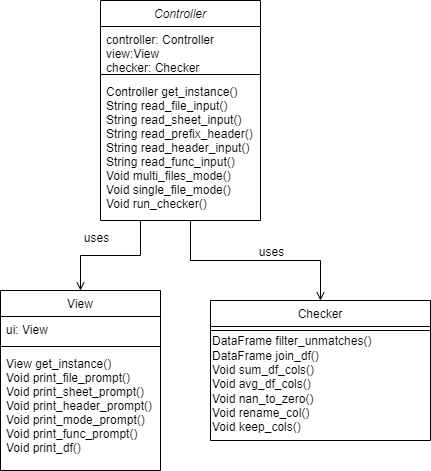
\includegraphics[width=0.7\textwidth]{UML_AutoChecker.png}
\end{center}

\medskip

\noindent The MVC design pattern are specified and implemented in the following way: 
the module \textit{BoardT} stores the state of the game board, the abstract 
object \textit{GameStatus} determines the status of the game.A view module 
\textit{View} displays the game board and the state of the game using a 
text-based graphics. The controller \textit{Controller} is responsibe for 
handling input actions

\medskip

\noindent For \textit{View} and \textit{Controller}, use the get\_instance() method to obtain the abstract object.

\newpage

\section* {Checker Module (Abstract Object)}

\subsection*{Module}

Checker

\subsection* {Uses}

None

\subsection* {Syntax}

\subsubsection* {Exported Constants}

None

\subsubsection* {Exported Types}

Checker = ?

\subsubsection* {Exported Access Programs}

\begin{tabular}{| l | l | l | p{5cm} |}
\hline
\textbf{Routine name} & \textbf{In} & \textbf{Out} & \textbf{Exceptions}\\
\hline
get\_unmatches & $\text{seq of } \mathbb{N}$, $\text{seq of } \mathbb{N}$ & $\text{seq of (seq of } \mathbb{N} \text{)}$ & \\
\hline
agg\_cols & $\text{seq of (seq of } \mathbb{N} \text{)}$, $\text{seq of } \mathbb{N} \rightarrow \mathbb{N}$ & $\text{seq of } \mathbb{N}$ & \\
\hline
trans\_mat & $\text{seq of (seq of } \mathbb{N} \text{)}$ & & \\
\hline

\end{tabular}

\subsection* {Semantics}

\subsubsection* {State Variables}

None

\subsubsection* {State Invariant}

None

\subsubsection* {Assumptions}

\begin{itemize}
  \item Every row that is being compared correspond to the same app prefix
  \item The number of rows that are being compared between columns are equal
\end{itemize}

\subsubsection* {Access Routine Semantics}

\noindent get\_unmatches(col1, col2):
\begin{itemize}
    \item output: out $:= [ i: \mathbb{N} | i \in \{0 .. |\text{col}1|-1\} : \text{col}1[i] \neq \text{col}2[i] \Rightarrow [ i,  \text{col}1[i], \text{col}2[i]] ]$
    \item exception: none
\end{itemize}

\noindent agg\_cols(cols, func):
\begin{itemize}
    \item output: out $:= [ i: \mathbb{N} | i \in \{0 .. |\text{cols}|-1\} : \text{func(cols}[i]\text{)} ]$
    \item exception: none
\end{itemize}

\noindent trans\_mat(matrix):
\begin{itemize}
    \item transition: $\forall i : \mathbb{N} \; | \; i < |\text{matrix}| $ $\wedge$ 
    ($\forall j : \mathbb{N} \; | \; i \le j < |\text{matrix}[i]|$ $\wedge$ tr\_swap($i$, $j$))
    \item exception: none
\end{itemize}

\subsubsection*{Local Function:}

% \noindent transMat: seq of (seq of $\mathbb{N}$)\\
% transMat(matrix): $\forall$ $i : \mathbb{N}$ $|$ $i < |\text{matrix}| $ $\wedge$ 
% ($\forall$ $j : \mathbb{N}$ $|$ $i \le j < |\text{matrix}[i]|$ $\wedge$ $\text{trSwap}(i, j)$)\\

\noindent tr\_swap: seq of (seq of $\mathbb{N}$) $\times \mathbb{N} \times \mathbb{N} \rightarrow$ void\\
\noindent tr\_swap(matrix, row, col): 
\begin{itemize}[\null]
  \item tmp $:=$ matrix[row][col]
  \item matrix[row][col] $:=$ matrix[col][row]
  \item matrix[col][row] $:=$ tmp
\end{itemize}

\newpage

\section* {View Module}

\subsection*{Module}

View

\subsection* {Uses}

None

\subsection* {Syntax}

\subsubsection* {Exported Constants}

None

\subsubsection* {Exported Types}

None

\subsubsection* {Exported Access Programs}

\begin{tabular}{| l | l | l | p{5cm} |}
  \hline
  \textbf{Routine name} & \textbf{In} & \textbf{Out} & \textbf{Exceptions}\\
  \hline
  get\_instance &  & View & \\
  \hline
  print\_file\_prompt & &  & \\
  \hline
  print\_sheet\_prompt & & & \\
  \hline
  print\_header\_prompt & & & \\
  \hline
  print\_mode\_prompt & & & \\
  \hline
  print\_mat & $\text{seq of (seq of } \mathbb{N} \text{)}$ & & \\
  \hline

\end{tabular}

\subsection* {Semantics}

\subsection*{Environment Variables}

window: A portion of computer screen to display the messages (i.e. the terminal)

\subsubsection* {State Variables}

ui: View

\subsubsection* {State Invariant}

None

\subsubsection* {Assumptions}

\begin{itemize}
  \item The View constructor is called for each object instance before any 
  other access routine is called for that object.  
  \item The constructor can only be called once.
\end{itemize}


\subsubsection* {Access Routine Semantics}

\noindent get\_instance( ):
\begin{itemize}
\item transition: ui $:=$ (ui = null $\Rightarrow$ new View())
\item output: \textit{self}
\item exception: none
\end{itemize}

\noindent print\_file\_prompt( ):
\begin{itemize}
\item transition: window $:=$ Displays a prompt message asking the user to enter a file directory
\end{itemize}

\noindent print\_sheet\_prompt( ):
\begin{itemize}
\item transition: window $:=$ Displays a prompt message asking the user to enter a sheet name
\end{itemize}

\noindent print\_header\_prompt( ):
\begin{itemize}
\item transition: window $:=$ Displays a prompt message asking the user to enter a header name
\end{itemize}

\noindent print\_mode\_prompt( ):
\begin{itemize}
\item transition: window $:=$ Displays a prompt message asking the user to select a checker mode
\end{itemize}

\noindent print\_mat( ):
\begin{itemize}
\item transition: window $:=$ Displays the matrix row by row
\end{itemize}

\subsubsection*{Local Function:}

\_\_init\_\_: void $\rightarrow$ View \\
\_\_init\_\_() $\equiv$ new View()

\newpage

\section* {Controller Module}

\subsection* {Controller Module}

\subsection* {Uses}

Checker, View, pandas

\subsection* {Syntax}

\subsubsection* {Exported Types}

None

\subsubsection* {Exported Constants}

None

\subsubsection* {Exported Access Programs}

\begin{tabular}{| l | l | l | p{4.7cm} |}
\hline
\textbf{Routine name} & \textbf{In} & \textbf{Out} & \textbf{Exceptions}\\
\hline
get\_instance & View & Controller & \\
\hline
read\_file\_input & & String & \\
\hline
read\_sheet\_input & & String & \\
\hline
read\_header\_input & & String & \\
% \hline
% load\_xlsx & Strint, String & DataFrame & FileNotFoundException \\ 
%            &                &           & SheetNotFoundException \\ 
%            &                &           & FileNotSupportException \\
\hline
multi\_file\_mode & Map of String and String & &\\
                  & Pair of String and Map &  & \\
\hline
single\_file\_mode & Pair of String and Map & &\\
                   & Pair of String and Map & & \\
\hline
run\_checker & & & \\
\hline
\end{tabular}

\subsection* {Semantics}

\subsection*{Environment Variables}

None

\subsubsection* {State Variables}

view: View \\
controller: Controller

\subsubsection* {State Invariant}

None

\subsubsection* {Assumptions}

\begin{itemize}
  \item The Controller constructor is called for each object instance before any
  other access routine is called for that object.  
  \item The constructor can only be called once.
  \item Assume that the view instances are already initialized before calling 
  Controller constructor
\end{itemize}

\subsubsection* {Access Routine Semantics}

get\_instance($v$):
\begin{itemize}
  \item transition: controller $:=$ (controller = null $\Rightarrow$ new Controller ($v$))
  \item output: \textit{self}
  \item exception: None
\end{itemize}

\noindent read\_file\_input():
\begin{itemize}
  \item output: $input$ : String, file directory entered by the User
  \item exception: none
\end{itemize}

\noindent read\_sheet\_input():
\begin{itemize}
  \item output: $input$ : String, sheet name entered by the User
  \item exception: none
\end{itemize}

\noindent read\_header\_input():
\begin{itemize}
  \item output: $input$ : String, column header entered by the User
  \item exception: none
\end{itemize}

\noindent read\_mode\_input():
\begin{itemize}
  \item output: $input$ : String, mode selected by the User
  \item exception: none
\end{itemize}

\noindent single\_file\_mode(file1, file2):
\begin{itemize}
  \item transition: operational method 
  \begin{itemize}[\null]
    \item arr1 $:=$ get\_col\_arr(file1[$0$], file1[$1$])
    \item arr2 $:=$ get\_col\_arr(file2[$0$], file2[$1$])
    \item unmatches\_rows $:=$ Checker.get\_unmatches(arr1, arr2)
    \item view.print\_mat(unmatches\_rows)
  \end{itemize}
  \item output: none
\end{itemize}

\noindent multi\_files\_mode(f\_map, file2):
\begin{itemize}
  \item transition: operational method 
  \begin{itemize}[\null]
    \item f\_arr $:=$ [$f$:String $|$ $f \in$ f\_map.keys() $:$ get\_col\_arr($f$, f\_map[$f$]) ]
    \item Checker.trans\_mat(f\_arr)
    \item arr1 $:=$ Checker.agg\_cols(f\_arr)
    \item arr2 $:=$ get\_col\_arr(file2[$0$], file2[$1$])
    \item unmatches\_rows $:=$ Checker.get\_unmatches(arr1, arr2)
    \item view.print\_mat(unmatches\_rows)
  \end{itemize}
  \item output: none
\end{itemize}

\noindent run\_checker():
\begin{itemize}
  \item transition: operational method for running the game. \\
  Start by prompting the user to select the checker mode (single file vs multi files)
  \begin{itemize}
    \item If single file mode is selected:
      \begin{itemize}[\null]
        \item $f1$ $:=$ () 
        \item $f2$ $:=$ ()
        \item populate\_pair($f1$)
        \item populate\_pair($f2$)
        \item single\_file\_mode($f1$, $f2$)
      \end{itemize}
    \item If multi files mode is selected:
      \begin{itemize}[\null]
        \item $f\_map$ $:=$ \{\}
        \item $f1$ $:=$ () 
        \item populate\_pair($f1$)
        \item inputs $:=$ get\_inputs()
        \item f\_map[inputs[$0$]] $=$ \{'sheet':inputs[$1$], 'header':inputs[$2$]\}
        \item populate f\_map by repeating step $3$ - $4$ five times
        \item multi\_files\_mode($f\_map$, $f1$)
      \end{itemize}
  \end{itemize}

  \item output: None
\end{itemize}

\subsubsection*{Local Function:}

\_\_init\_\_: View $\rightarrow$ Controller \\
\_\_init\_\_($view$) $\equiv$ new Controller($view$) \\

% $\text{tmp} = \text{matrix}[row][col] \ \wedge \  
% \text{matrix}[row][col] = \text{matrix}[col][row] \ \wedge \ 
% \text{matrix}[col][row] = \text{tmp}$\\

\noindent cal\_sum: seq of $\mathbb{N} \rightarrow \mathbb{N}$\\
cal\_sum(seq) $\equiv (+s:\mathbb{N} \; | \; s \in \text{seq} : s)$ \\

\noindent cal\_avg: seq of $\mathbb{N} \rightarrow \mathbb{N}$\\
cal\_avg(seq) $\equiv \text{cal\_sum}(seq) / |\text{seq}|$\\

\noindent get\_col: String $\times$ Map of String and String $\rightarrow$ seq of $\mathbb{N}$\\
get\_col\_arr(file\_dir, info\_map):
\begin{itemize}[\null]
  \item df $:=$ load\_xlsx(file\_dir, info\_map['sheet'])
  \item return df[info\_map['header']].values
\end{itemize}

% \noindent col\_to\_arr: Series $\rightarrow$ seq of $\mathbb{N}$\\
% col\_to\_arr(df\_col) $\equiv$ df\_col.values\\

% \noindent get\_df\_col: DataFrame $\times$ String $\rightarrow$ Series\\
% get\_df\_col(df, header) $\equiv$ df[header]\\

\noindent get\_inputs: seq of String\\
get\_inputs(p): 
\begin{itemize}[\null]
  \item view.print\_file\_prompt()
  \item file\_dir $:=$ read\_file\_input()
  \item view.print\_sheet\_input()
  \item sheet $:=$ read\_sheet\_input()
  \item view.print\_header\_input()
  \item header $:=$ read\_header\_input()
  \item return [file\_dir, sheet, header]
\end{itemize}

\noindent populate\_pair: Pair $\rightarrow$ void\\
populate\_pair(p): 
\begin{itemize}[\null]
  \item inputs $:=$ get\_inputs()
  \item $p[0] :=$ inputs[$0$]
  \item $p[1] :=$ {'sheet':inputs[$1$], 'header':inputs[$2$]}
\end{itemize}

\noindent load\_xlsx: String $\times$ String $\rightarrow$ DataFrame
load\_xlsx(file\_dir, sheet\_name) $\equiv$ pandas.read\_excel(file\_dir, sheet\_name)

\end {document}